\documentclass[a4paper,12pt]{article} % тип документа
\usepackage[margin=1in]{geometry} % Поля

%  Русский язык
\usepackage[warn]{mathtext}
\usepackage[T2A]{fontenc}			% кодировка
\usepackage[utf8]{inputenc}			% кодировка исходного текста
\usepackage[english,russian]{babel}	% локализация и переносы
% Математика
\usepackage{amsmath,amsfonts,amssymb,amsthm,mathtools} 
\usepackage{wasysym}
%%%
\usepackage{graphicx}

\usepackage{tabularx}

\usepackage{gensymb} % знак градуса
\usepackage{enumitem} % изменить список enumerate
\usepackage{placeins} % \FloatBarrier

\renewcommand{\thesection}{\Roman{section}} 
\renewcommand{\thesubsection}{\roman{subsection}}


\begin{document}

\newcolumntype{Y}{>{\centering\arraybackslash}X} %new tabularx


%титул
\hrule 	
\medskip
\begin{raggedright}
{\large \textbf{Отчёт по работе 5.1.2}}
\\
\medskip
{\Large Исследование эффекта Комптона} 
\\
\medskip
{\large Карташов Констанин Б04-005}
\medskip
\hrule
\medskip
\end{raggedright}


\section{Анотация}

\paragraph{Цель работы:} 
Исследовать энергетический спектр $\gamma$--квантов, рассеянных на графите. Определение энергии рассеянных $\gamma$--квантов в зависимости от угла рассеяния, а также энергия покоя частиц, на которых происходит рассеяние.

\paragraph{Оборудование:}
\begin{itemize}
\renewcommand{\labelitemi}{$\triangleright$}
\itemsep0em
\item Сцинтилляционный спектрометр
\item Источник направленного $\gamma$--излучения
\item Графитовая мишень
\end{itemize}


\medskip\hrule\medskip

\section{Теоретическая часть}

\subsection{Необходимые формулы}

\paragraph{} Эффектом Комптона называется рассеяние фотона заряженной частицей, приводящее к уменьшению его энергии, и соответствующим увеличением длины его волны. В нашем случае $\gamma$--квант испускаемый цезием 137 рассеивается об электроны в графитовом цилиндре. Данный эффект не объясняется классической электродинамикой, для его объяснения необходимо считать взаимодействие фотона и электрона упругим соударением.

\paragraph{} Из расчёта абсолютно упругого соударения фотона и электрона, используя закон сохранения импульса и энергии получим формулу для изменения длины волны рассеянного $\gamma$--кванта:

\begin{equation}
\Delta \lambda = \lambda_1 - \lambda_0 = \frac{h}{mc}(1 - \cos{\theta}) = \Lambda_{K}(1 - \cos{\theta}), 
\label{e:e1}
\end{equation}

\noindent где $\Lambda_{K} = \frac{h}{mc} = 2.42 \cdot 10^{-10}$ см -- комптоновская длина волны электрона.

Подставив в формулу (\ref{e:e1}) энергию $\gamma$--кванта $\varepsilon = \hbar \omega$ получим другую форму записи:

\begin{equation}
\frac{1}{\varepsilon(\theta)} - \frac{1}{\varepsilon_0} = 1 - \cos{\theta}.
\label{e:e2}
\end{equation}

\subsection{Экспериментальная установка}

\begin{figure}[h]
\centering
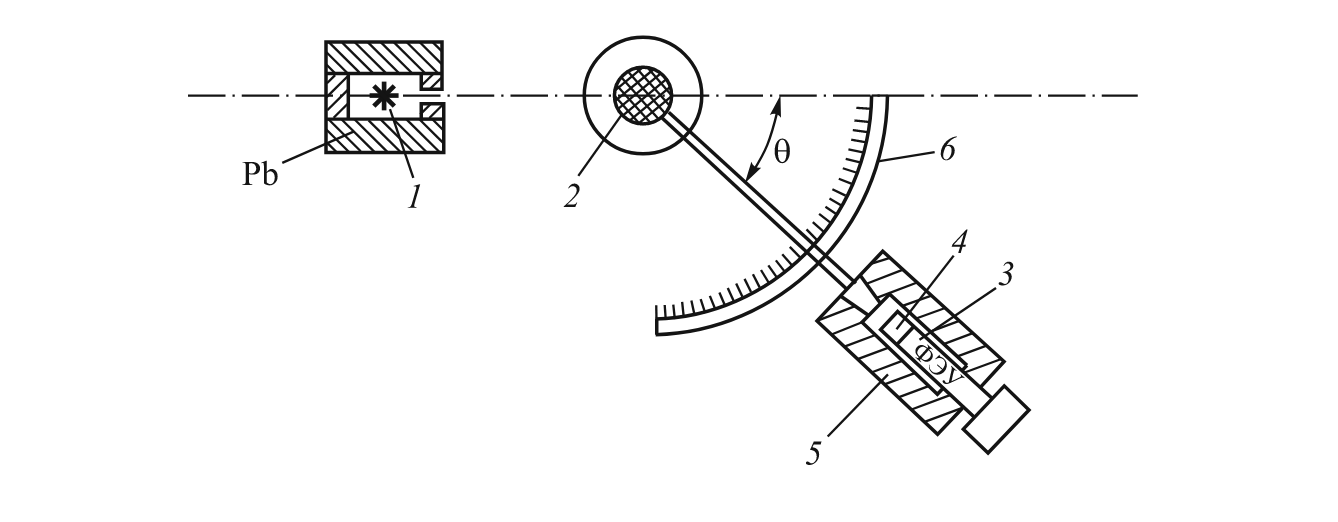
\includegraphics[width=\textwidth]{setup.png}
\caption{Схема экспериментальной установки}
\label{fig:setup}
\end{figure}

\paragraph{} Экспериментальная установка (рис. \ref{fig:setup}) состоит из:
\begin{enumerate}
\itemsep0em
\item Источника излучения $^{137}$Cs, помещённого в свинцовый контейнер с коллиматором.
\item Графитовой мишени в форме цилиндра. 
\item Фотоэлектронного умножителя.
\item Кристалла NaI(Ti), выполняющего роль сцинтиллятора.
\item Свинцового коллиматора.
\item Лимб для расчёта угла рассеяния.
\end{enumerate}

\paragraph{} ФЭУ и сцинтиллятор образуют сцинтилляционный счётчик, который подключается к усилителю-анализатору, который фиксирует попадание $\gamma$--кванта в счётчик, и передаёт значение его энергии на компьютер в 1024 дискретных уровнях (каналах), номер которых $N$ прямо пропорционален значению энергии. На экране компьютера выводиться гистограмма всех зафиксированных попаданий в каждом из каналов.

\medskip\hrule\medskip

\section{Экспериментальная часть}

\subsection{Проведение измерений}

\paragraph{} При помощи экспериментальной установки измерим зависимость номера фотопика $N$ от положения сцинтилляционного счётчика $\theta$. В качестве номера фотопика возьмём номер наибольшого столбца в гистограмме, соответствующего к пику созданным рассеянными фотонами. Полученные данные приведены в таблице \ref{tab:data}.

\begin{table}[h]
\centering
\begin{tabular}{|c|c|c|c|c|c|c|c|c|c|c|c|c|c|c|}
\hline
$\theta$\degree & 0   & 10  & 20  & 30  & 40  & 50  & 60  & 70  & 80  & 90  & 100 & 110 & 120 & 130 \\ \hline
$N$      & 897 & 893 & 845 & 689 & 683 & 560 & 488 & 421 & 383 & 345 & 313 & 280 & 261 & 246 \\ \hline
\end{tabular}
\caption{Значение угла в градусах и соответствующий фотопик.}
\label{tab:data}
\end{table}


\subsection{Обработка данных}

\paragraph{} Учитывая то, что номер канала фотопика прямо пропорционален энергии кванта зафиксированного счётчиком, заменим в формуле (\ref{e:e2}) энергию $\varepsilon$ номером канала максимума фотопика $N$, и добавив неизвестный коэффициент пропорциональности $A$, получим формулу:

\begin{equation}
\frac{1}{N(\theta)} - \frac{1}{N(0)} = A(1 - \cos{\theta}).
\label{e:e3}
\end{equation}

\paragraph{} Для более удобной обработки измеренных данных (табл. \ref{tab:data}), построим график зависимости $1 - \cos{\theta}$ от $1/N(\theta)$, и проведём через полученные точки наилучшею прямую (по МНК) (рис. \ref{fig:plot}). 

\begin{figure}
\centering
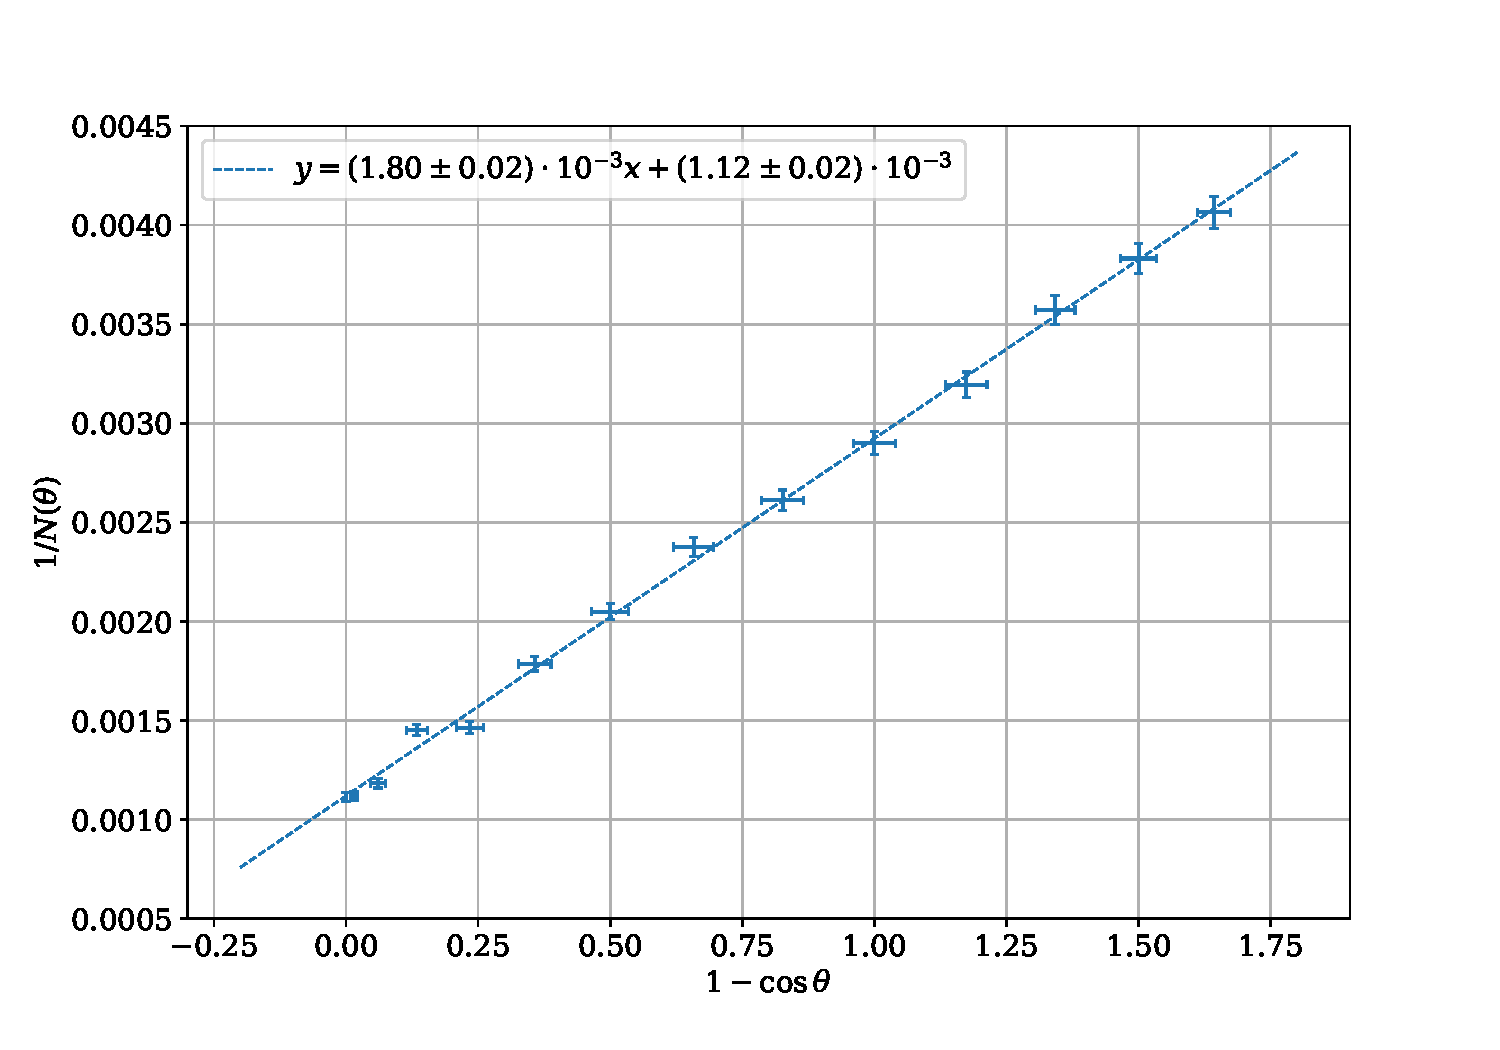
\includegraphics[width=\textwidth]{plot_2.pdf}
\caption{График измеренных значений и наилучшей прямой}
\label{fig:plot}
\end{figure}

По наилучшей прямой определим наилучшие значения для $N$ при $\theta = 0\degree$ и $\theta = 90\degree$, получим:

\[
\theta = 0\degree \; \Rightarrow \; x = 0 \; \Rightarrow y(0) = (1.12 \pm 0.02) \cdot 10^{-3},
\]\[
N(0) = \frac{1}{y(0)} = 893, \; \Delta N(0) = N(0) \cdot \frac{\Delta y(0)}{y(0)} = 16, \; N_\text{наил}(0) = 890 \pm 20;
\]\[
\theta = 90\degree \; \Rightarrow \; x = 1 \; \Rightarrow y(1) = (2.92 \pm 0.04) \cdot 10^{-3},
\]\[
N(90) = \frac{1}{y(1)} = 342, \; \Delta N(90) = N(90) \cdot \frac{\Delta y(1)}{y(1)} = 5, \;
N_\text{наил}(90) = 342 \pm 5.
\]

\subsection{Проверка результатов}

\paragraph{} Воспользуемся формулой (\ref{e:e2}), подставив значение $\theta = 90\degree$:

\[
mc^2 \left( \frac{1}{E(90)} - \frac{1}{E(0)} \right) = 1,
\]

\noindent или

\[
mc^2 = E(0)\frac{E(90)}{E(0) - E(90)} = E_\gamma \frac{N(90)}{N(0) - N(90)},
\]

\noindent где $E_\gamma$ -- энергия электронов, рассеянных вперёд, или просто энергии $\gamma$--лучей.

\paragraph{} Теперь найдём энергию покоя частицы $E_\text{П} = mc^2$, рассчитанной по формуле:

\[
E_\text{П} = E_\gamma \frac{N_\text{наил}(90)}{N_\text{наил}(0) - N_\text{наил}(90)} = 662 \text{ кэВ} \cdot \frac{342}{890 - 342} = 413 \text{ кэВ},
\] \[
\Delta E_\text{П} = E_\text{П} \cdot \sqrt{2 \left( \frac{\Delta N(90)}{N(90)} \right)^2 + \left( \frac{\Delta N(0)}{N(0)} \right)^2} = 13 \text{ кэВ}.
\]

Получили $mc^2 = 410 \pm 20$ кэВ, что значительно ниже действительного значения $mc^2 = 511$ кэВ.

\medskip\hrule\medskip

\section{Выводы}

\begin{enumerate}
\item Пронаблюдали эффект Комптона при помощи сцинтилляционного счётчика, заметив изменение энергии рассеянных $\gamma$--квантов при изменении угла рассеяния.
\item Подтвердили состоятельность формулы (\ref{e:e1}) и её вывода, получив прямую зависимость на графике (рис. \ref{fig:plot}).
\item Посчитали энергию покоя электронов, рассеивающих $\gamma$--кванты, получив значение $mc^2 = 410 \pm 20$ кэВ, что на $20\%$ отличается от действительного значения $mc^2 = 511$ кэВ. Это различие можно объяснить неточностью при определении номера канала $N$, соответствующего фотопику.
\end{enumerate}

\medskip\hrule\medskip

\end{document}
